%bNEWSystemTest
%test
\section{System test}
This section covers the test of the system, prior to conducting the experiment for the project. 

\subsection{Method of test for gyroscopes}
The authors assess that a test of the gyroscopes is not necessary, as the Shimmer3 devices will be calibrated using the built in function of Shimmer Sensing’s program, Consensys, to ensure the devices are working as expected.

%til test af gyro/accel kan vi gøre som paul foreslog og filme personen imens de drejer rundt eller noget, hvor vi kan synkronisere film med gyro/accel målinger og se at der sker udsving på samme tidspunkt som personen drejer/bevæger sig. Det kan self ikke være med i rapporten men vi kan vise det til eksamen. 


\subsection{Method of test for Force Sensitive Resistors}
The FSR will be tested by placing a 1-2 kg weight covering a surface area of “insert cm2” on the 402 sensors and “insert cm2” on the 406 sensors and measuring the resulting resistance with a “insert voltmeter name here”. This is done to ensure that none of the sensors are either broken or deviate compared to the mean result of the test. 

%retfærdigøre at vi brugere sensore der "kun" kan måle så lidt tryk til at måle under folk som vejer +50 kg. Sikkert noget med at simon har sat modstande i systemet som øger sensorernes måling af tryk påvirkning. 

\subsection{Test  results for Force Sensitive Resistors}

Everything was *hopefully*fine. 



\subsection{System test}
The system as a whole will be tested with a walk sequence. The sequence will involve periods of no movement, movement by walking and turning and a light jump to mark the beginning and end of the sequence. The walk sequence is as follows:
\begin{itemize}
	\item Start
	\item 3 second pause
	\item Light jump
	\item 1 second pause
	\item Walk five steps
	\item 180 degree turn
	\item Walk five steps
	\item 1 second pause
	\item Light jump
	\item 3 second pause
	\item End
\end{itemize}
%Test walk sequence: Wait 3 sec. light jump. wait 1 sec. walk 5 steps. 180 turn. walk 5 steps. 90 turn right. wait. 90 turn right. wait. quick 180. wait quick 180. wait 1. light jump. wait 3 sec. 
Following the system test the acquired data will be qualitatively evaluated to ensure everything works as intended. 

\subsection{Test results for System test}
Everything was fine. 

%sensor bait text fra DataAcquisition.tex
A problem occurred with the FSR 406 placed under the heel of the subject during the system test . When weight was applied to the sensor it would measure the highest possible force the sensor can measure, and no useful data could be collected from the sensor. It was evaluated why this happened and discovered that because the FSR 406 covers a larger area and were placed at the heel it would be affected by more force when a subject stood on it. As the distribution of pressure is higher at the heel compared to anywhere else under the foot while standing, it makes sense that the FSR 406 would be overloaded \cite{Hessert2005}. To account for this, the FSR 402 placed at the lateral side of the feet where switched with the FSR 406 at the heel. As the FSR 402 covers a smaller area they would not be overloaded as easily as the FSR 406. As a result the FSR 406 is now placed at the lateral side of the eminence of the sole, and one FSR 402 is placed at the heel. The new placement of FSR sensors can be seen in \figref{fig:soleSensorPlacement}.

\begin{figure}[H]
	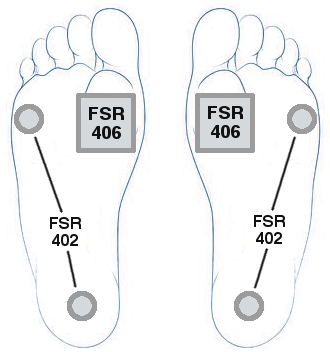
\includegraphics[width=.6\textwidth]{figures/humanSoleSensorPlacement}
	\caption{The new placement of the FSR 402s and 406 under the foot of subjects.}
	\label{fig:soleSensorPlacement}  %<--remember LABEL!
\end{figure}

With the new placement of the FSR’s the system functions as intended and is ready for the experiment. 
